\section{Holographic Visualization}
\label{sec.holographic_visualization}

The holographic display is a new generation of 3D display technology pursued by many researchers~\cite{Lucente1992, Watlington1995, Lucente2012} and companies~\cite{schwerdtner2013} over the past decades. Those works use special displays to create the holographic effect of the incident of a source beam of light on a fringe pattern. This is later rendered using CGH, but the necessary amount of data for real-time rendering is not feasible for using today's technology. For example, a 60-cm-diagonal hologram has over $10^{12}$ samples --– the equivalent of a terabyte~\cite{Lucente2012}. While promising technologies have been proposed lately to decimate the amount of data~\cite{Lucente1992, schwerdtner2013}, there is a gap in the currently established 3D display technology and processing power for quality holograms. 

Holograms are expected to show visual effects of a 3D scene as a Volume Of Interest (VOI) projected outside the screen. The projection keep all the depth cues of the objects of the VOI: the relative sizes of the objects from the perspective deformation, the stereo depth perception from stereo convergence, binocular parallax and ocular accommodation of the eyes by focusing at different distances; the motion parallax~\cite{li2012} from the difference in the positions of the objects as the viewer moves, the monocular occlusion~\cite{Lucente1995} when one part of image is obstructed by another overlapping part; and pictorial monocular depth cues of texture gradient, aerial perspective, shading, and relative sizes~\cite{Lucente1995}. 

The hologram has a unique feature: viewers are allowed to walk around the VOI and have a \emph{surround viewing}~\cite{debevec2006}, a shared visualization in different angles that is naturally perceived by the eyes without any wearable apparatus. Additionally to that, two or more viewers can view the VOI in different angles because the viewing rays are propagated in a Field of View (FOV) from the holographic apparatus~\cite{Lucente1992}. The current CGH displays have a limited FOV of $60^{\circ}$~\cite{Slinger2005, Lucente1995} due the compromise of the quality of the hologram and computational processing power.

The surround viewing, combined with the depth cues, creates the illusion effect of Pepper's Ghost~\cite{smithwick2014}, which means that the viewer can interact with the VOI with no physical barriers. The practical applications for the combined 3D visualization and interaction can be illustrated, but not limited, in Medical Imaging. For example, a scene of 3D reconstructed organs from 3D medical imagery of 3D Computed Tomography (CT) scans or Magnetic Resonance Imaging (MRI) composes the VOI and is projected as a hologram. The organs are the objects that can be manipulated \emph{in locus} for virtual surgery, and there is no display screen acting as a physical barrier between the object and viewer. Any examination of the organs is provided by the surround viewing and depth cues of the VOI. The surgery simulation is achieved because the spectral illusion is created for the surgeon in a Virtual Reality (VR) environment.

\subsection {Holographic Emulation}
\label{sec.holographic_emulation}

The proposal of this work is to investigate a Virtual Reality (VR) environment that can provide the combined effects of the hologram but that don't have the computational cost of CGH. Most of current VR environments can be composed of off-the-shelf hardware, and the proposed environment does not rely on specialized hardware for CGH to avoid its high costs~\cite{fournier2004}. The proposed VR environment is composed by two 3D standard stereo TVs, combined in a Fish Tank Virtual Reality (FTVR)~\cite{Ware1993} environment and a depth camera. The camera creates a Head Coupled Perspective (HCP)~\cite{okoshi2012}, as shown in Figure~\ref{fig.tv_setup}, by projecting virtual objects considering the location of the viewer, which is acquired by tracking. HCP improves the depth perception~\cite{li2012} and, when combined with stereo vision, can create an holographic emulation. 

The FTVR is combined with HCP and stereo vision to create a virtual screen, which is the perceived screen from the depth cues created by the two stereo displays that are juxtapositioned with a tilt angle of in Figure~\ref{fig.tv_setup}. The surround viewing is achieved by tracking the position of the viewer as in the original FTVR setup. Although HCP is has been reported more important than stereo in 3D visualization~\cite{Ware1993}, the holographic perception is created using the binocular parallax. The HCP viewing is adjusted with negative parallax to create the depth cue of the virtual screen and the spectral illusion of Pepper's Ghost. Other depth cues are adjusted to the viewing angle of the virtual screen using the position tracked by the the depth camera.

\begin{figure}[!hbt]
\centering
%\begin{tabular}{cc}
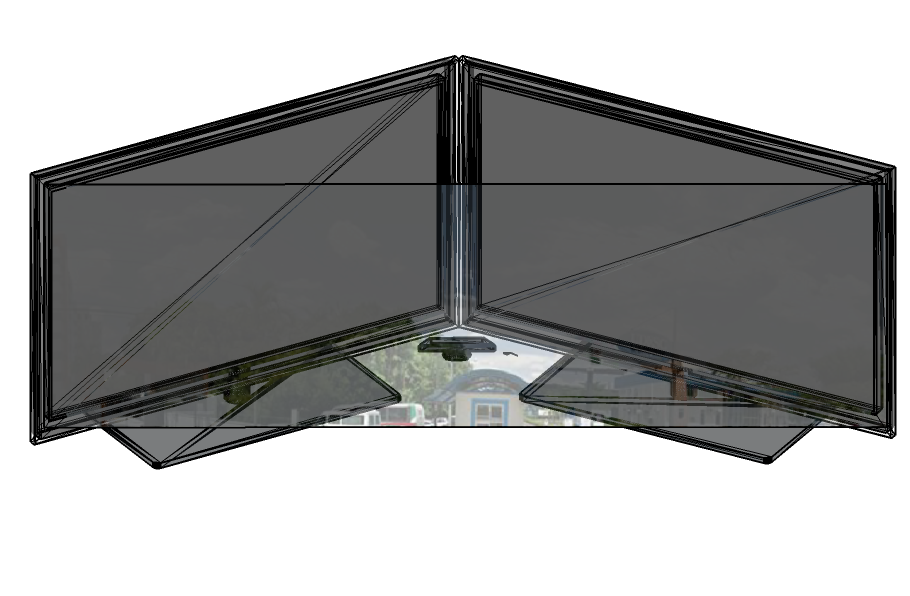
\includegraphics[width=\linewidth,keepaspectratio=true]{figs/labsetup_01.png}
%&
%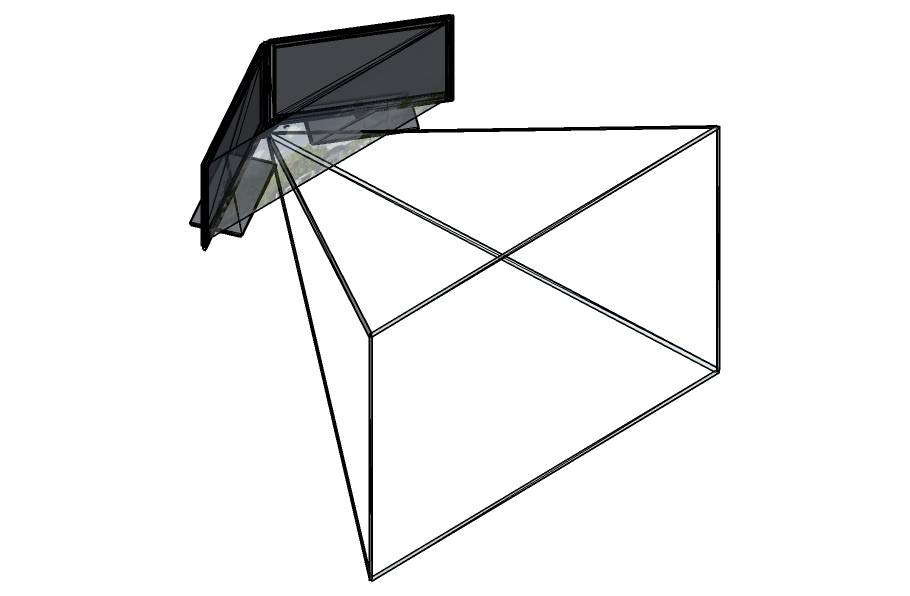
\includegraphics[width=0.4\linewidth,keepaspectratio=true]{figs/labsetup_02.png}\\
%(a) Virtual screen & 
%(b) Tracking frustum
%\end{tabular}
\caption{FTVR setup of the stereo displays and depth camera.}
\label{fig.tv_setup}
\end{figure}

The tracking system has to capture the position of the viewer with high accuracy in order to avoid incorrect HCP. It also needs to be robust to body movement or objects that may partially occlude the viewer. In order to achieve the desired robustness and accuracy, a depth camera is used instead of a standard RGB camera. The depth sensor has a higher accuracy in the estimation of the depth and with this information can remove artifacts in the image that are occluding or degrading the positional information of obtained from the RGB channels. 

Although the proposed emulation has the restriction of a single viewer for simplicity, the proposed setup can be extended up to four viewers. The depth information can be also used to distinguish two people in front of the TVs, and two depth cameras can be combined to track four viewers. The standard stereo TVs with 240 Hz refresh rate can provide stereo pairs up to four viewers with some flickering~\cite{Frohlich2005}. 

%This investigation setups two 3D displays forming the FTVR as in the illustration of Figure~\ref{fig.tv_setup}a. 



%The cornerstone of the proposed projection is how this can be done with the existing viewing pipeline of 3D graphics frameworks such as OpenGL. The existing viewing transformations works well for 3D with positive stereo parallax, showing the object as inside the screen of display. In the opposite case, the projection with negative parallax requires the translation $T_{parallax}$ of the scene towards the virtual display. This is incorporated in the view transformation $M_{view}$ of Section~\ref{sec.projection_review}, creating a translated view $M_{view}T$. Let the modification of the viewpoint produce a new view transform $M^{\prime}_{view}$. This new viewpoint combined with $T_{parallax}$ is then defined as $M^{\prime}_{view} T$. The following projection $M_{projection}$ depends on the value of $z$, which means that the latter translation is not applied not only in the depth, but also in the other directions, moving the scene coordinates with the distance from the screen. 

%In the proposed hologram emulation, the scene should be projected with negative parallax to appear in a distance away from the screen. For the viewer, objects of the scene appears in a fixed position outward from the screen. The immersion depends on the viewer position for eye accommodation, stereo convergence and binocular parallax. Additionally to that, the FOV provided by the FTVR and HCP projection enhances the realism of the scene and the sense of presence~\cite{Hounsell2013}. 

%The HCP projection of the scene provided by the OpenGL pipeline in Section~\ref{sec.projection_review} works for standard stereo projection. In the proposed hologram emulation, the projection has to emulate a virtual Volume Of Interest (VOI) with the stereo negative parallax. The VOI is created with depth cues to emulate the hologram. The perspective cue is dependent on the viewing angle and distance from screen, but not on binocular parallax. 

%There is no motion parallax in the VOI and all objects in the hologram have fixed position.

%The main pipeline of OpenGL follows the sequence of transforms: $M_{model}$, $M_{view}$, $M_{proj}$ and $M_{screen}$. In ordinary HCP, $M_{model}$ setups the scene. $M_{view}$ applies the viewpoint from the tracked position, and $M_{proj}$ sets the depth cues. While the perspective depth cue is set with $M_{proj}$, the binocular parallax is set with the stereo projection of Equation~\ref{eq.stereo_projection_matrix} in Section~\ref{sec.stereo_projection}. This projection has zero parallax for a convergence point in the plane of projection, which is the screen of display, and negative parallax at any convergence point in front of the stereoscopic displays. In order to achieve this, the view transform $M_{view}$ has to create a viewpoint looking towards $-z$, because the horizontal negative parallax has to increase away from the screen with the multiplication of the first term on the right of Equation~\ref{eq.stereo_projection_matrix} and the object coordinates $(x, y, z)$ in the VOI. The result of this multiplication is the coordinate translated in $x$ to create the stereo offset, $(x+ sh_z \cdot z, y, z)$. Therefore, the objects have increasing negative parallax in the increasing positive $z$ axis.

%This projective setup introduces a motion parallax for object that are off-center. This is desired for HCP with positive parallax, but not for the hologram emulation because the VOI does not have motion parallax associated with the viewpoint. If $M_view$ is restricted to invert the orientation of the $z$ axis, and $M_{proj}$ applies the shift in the frustum that aligns that origin with the plane with zero parallax, the far plane in most cases, the motion parallax of the HCP is removed. This also is incorrect  because $M_{view}$ should be applied after the shift to generate the viewpoint for HCP. If applied before, the viewpoint is for a scene that is projected along $-z$ as in glFrustum(). One possible way is to correct to keep $M_{view}$ fixed and adjust the rotation and position of each model $M_{model}$ in order to produce the correct viewing angle, but those are cumbersome operations that are not in the semantics of each transform in the OpenGL pipeline. 

%The Figures~\ref{fig.transformation}a-d show an example of a scene composed of duck 3D model. Figure~\ref{fig.transformation}a shows the scene with the shift its applied before the projection to create negative parallax. If the viewpoint is changed to look the top left corner of the picture, a motion parallax is created, illustrated in Figure~\ref{fig.transformation}b. If the shift is applied after $M_{proj}$, the motion and binocular parallaxes are correct, but not the HCP, and the duck in Figure~\ref{fig.transformation}c is not aligned with the viewpoint in the left top corner.The correct viewing angle, as shown in Figure~\ref{fig.transformation}d, can be adjusted programmatically with $M_{model}$ of each object in the scene.

% remove \iffalse ... \fi block to uncomment
\iffalse

\begin{figure}
\centering
\begin{tabular}{|c|c|}
\hline
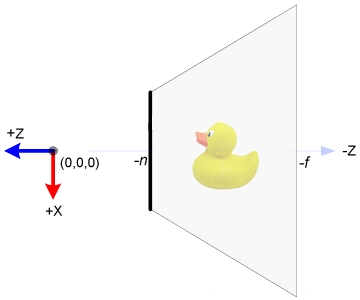
\includegraphics[width=0.45\linewidth,keepaspectratio=true]{figs/scene01.png}
&
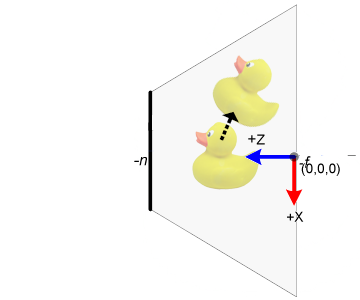
\includegraphics[width=0.45\linewidth,keepaspectratio=true]{figs/scene02.png}
\\
(a)&(b)\\ \hline
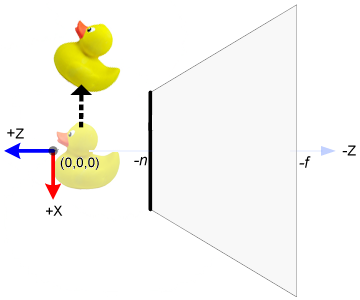
\includegraphics[width=0.45\linewidth,keepaspectratio=true]{figs/scene03.png}
&
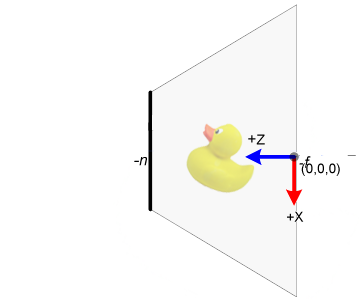
\includegraphics[width=0.45\linewidth,keepaspectratio=true]{figs/scene04.png}
\\ 
(c)&(d)\\ \hline
\end{tabular}
\caption{Example of a scene composed by a duck and the projection frustum of Section~\ref{sec.stereo_projection}. The viewer is at left center in picture (a)  and in the top left corner in pictures (b) to (d).}
\label{fig.transformation}
\end{figure}
\fi







\subsection{Holographic Pipeline}
\label{sec.holographic_pipeline}

The main pipeline presented in Section~\ref{sec.visualization_pipeline} follows the sequence of transforms: $M_{model}$, $M_{view}$, $M_{proj}$ and $M_{screen}$. In ordinary HCP, $M_{model}$ setups the scene. $M_{view}$ applies the viewpoint of the tracked position, and $M_{proj}$ sets the depth cues. The 3D viewing transforms, $M_{view}$ and $M_{proj}$ can be further split into smaller transforms: a \emph{view pipeline} and  a \emph{projection pipeline}, respectively.

In the proposed FTVR, the screens are tilted to create the virtual screen. The transformation matrix for the tilted screen-local coordinates, $M_{tilt}$, maps the Cartesian coordinate system of the virtual screen onto the screen space coordinate system. If a point is lying in the virtual plane, then the transformation $M_{tilt}$ will realign it to lie into the plane of the screen. The screen space basis are the vectors $v_r$, $v_u$, and $v_n$, the vectors for the right, up and normal directions. The mapping of $M_{tilt}$ is the inverse of the holographic mapping into the plane of the virtual screen. In the holographic views, any point lying in the plane of the screen will be realigned to lie in the virtual screen plane. This mapping is produced by the inverse of $M_{tilt}$. Fortunately, $M_{tilt}$ is an orthogonal rotation, and its inverse is its transpose, $M_{tilt}^{T}$, with screen space basis vectors as rows instead of as columns:

\begin{equation}
\begin{aligned}
M_{tilt}^{T} &= 
\begin{pmatrix} 
v_{rx} & v_{ry} & v_{rz} & 0\\
v_{ux} & v_{uy} & v_{uz} & 0\\
v_{nx} & v_{ny} & v_{nz} & 0\\
0      & 0      & 0      & 1\\
\end{pmatrix}
\end{aligned}
\label{eq.tilt_matrix_transpose}
\end{equation}

The viewpoint of the viewer, $M_{cam}$, simulates a camera looking towards $-z$. While the viewpoint can be applied anywhere in the 3D space, the mathematics of perspective projection as defined by matrix $M_{proj}$ disallow this, by the foreshortening division by $z$. The frustum of the camera is forever trapped at the origin, and if we wish to transform the viewpoint, we must instead apply the inverse of this transform to the entire scene. Thus, we instead align the scene with the frustum of the camera. The viewpoint of $M_{cam}$ has to be in tracked position $p_e$, then the scene is translated using the offset of the tracked position to the apex of the frustum. The apex of the perspective frustum is necessarily at zero, thus we translate by $-p_e$ along the vector from the eye:

\begin{equation}
\begin{aligned}
M_{cam} &= 
\begin{pmatrix} 
0      & 0      & 0      & -p_{ex}\\
0      & 0      & 0      & -p_{ey}\\
0      & 0      & 0      & -p_{ez}\\
0      & 0      & 0      & 1\\
\end{pmatrix}
\end{aligned}
\label{eq.camera_matrix}
\end{equation}

For the proposed HCP, the standard perspective transform is set as $M_{hcp}$. This transform have the same parallax for any convergence point in the plane of virtual screen. The near and far distances that composes $M_{hcp}$ are respectively set to the distances to: the plane of virtual screen and the center of the juxtaposition of the physical screens. 

The visualization pipeline for the left and right screens introduces independent transformations for each screen defined by projection transformations of each view. In usual cases, those projection transformations are used to create a wall composed by many juxtapositioned screens with a single vanishing point. The left and right distances in $M_{hcp}$ are displaced by an offset $s_o$. This offset transform $M_{off}$ is applied to $M_{hcp}$ in the projective pipeline $M_{proj} = M_{off} \times M_{hcp}$. In this pipeline,  $M_{hcp}$ transforms the scene coordinates to in NDC, as shown in Section~\ref{sec.visualization_pipeline}. Therefore the offsets for half screen to the left and right are $s_{ox} = -1$ and $s_{ox} = 1$, respectively. The offset transform $M_{off}$ have same form as $M_{eye}$, in Equation~\ref{eq.camera_matrix}, and is obtained replacing $-p_e$ by $s_o$.

In stereo visualization, the binocular parallax is obtained with the composition of $M_{eye}$ and $M_{stereo}$, Equations~\ref{eq.stereo_view_matrix} and~\ref{eq.stereo_proj_matrix}, in the view and projection pipelines. The view pipeline is the combination of the three transforms: $M_{view} = M_{tilt}^{T}   \times M_{eye} \times M_{cam}$. The plane of the virtual screen has a constant negative parallax at any convergence point in order to simulate the effect of Pepper's Ghost, as proposed in Section~\ref{sec.holographic_emulation}.  The shear transformation of $M_{stereo}$, Equation~\ref{eq.stereo_proj_matrix}, combined with a fixed offset $s_{oz}$ in $M_{off}$ creates constant negative parallax in the virtual screen. Thus, the projection pipeline becomes the combination of the three transforms: $M_{proj} = M_{stereo}  \times M_{off} \times M_{hcp}$. 

The stereo polarization each side of the left and right stereo pairs in Figures~\ref{fig.split_screens}a-b shows the views as projected in the virtual screen.

\begin{figure}[!hbt]
\centering
\begin{tabular}{cc}
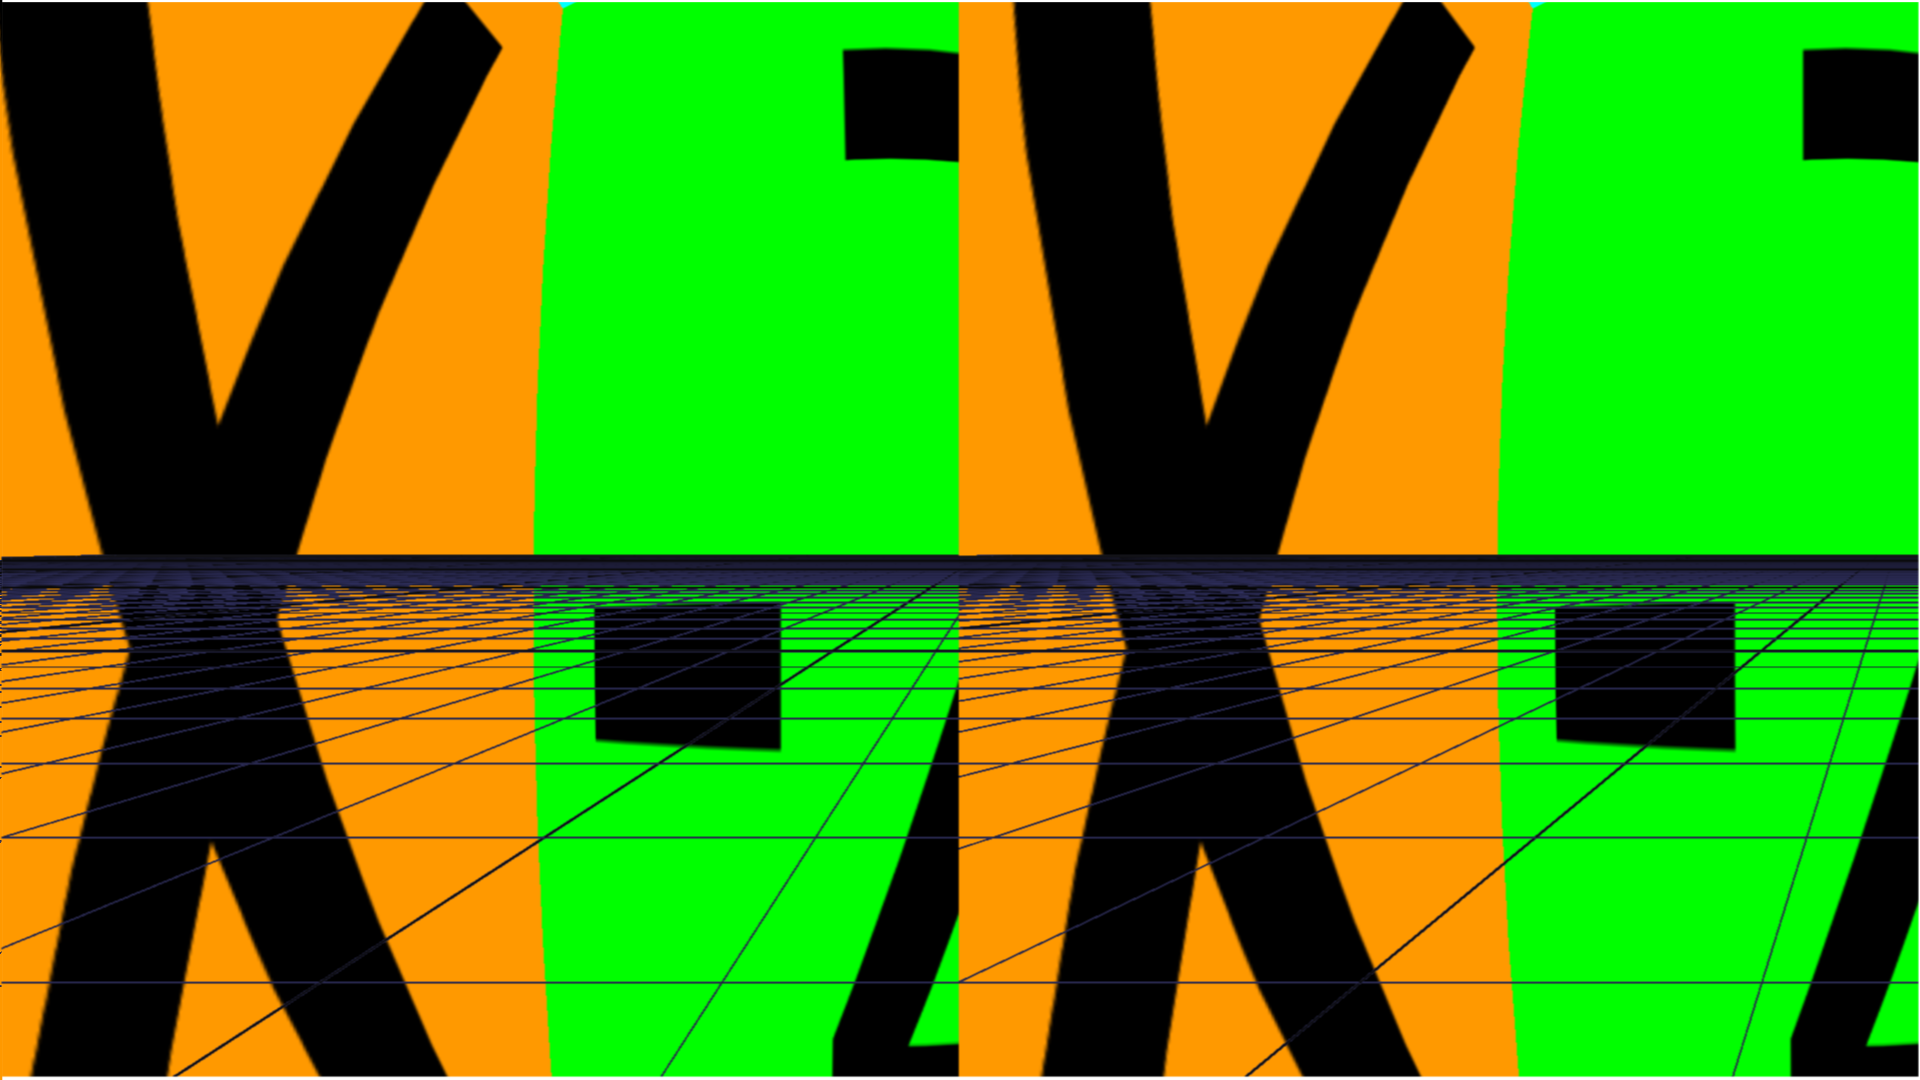
\includegraphics[width=0.45\linewidth,keepaspectratio=true]{figs/left_screen.png}&
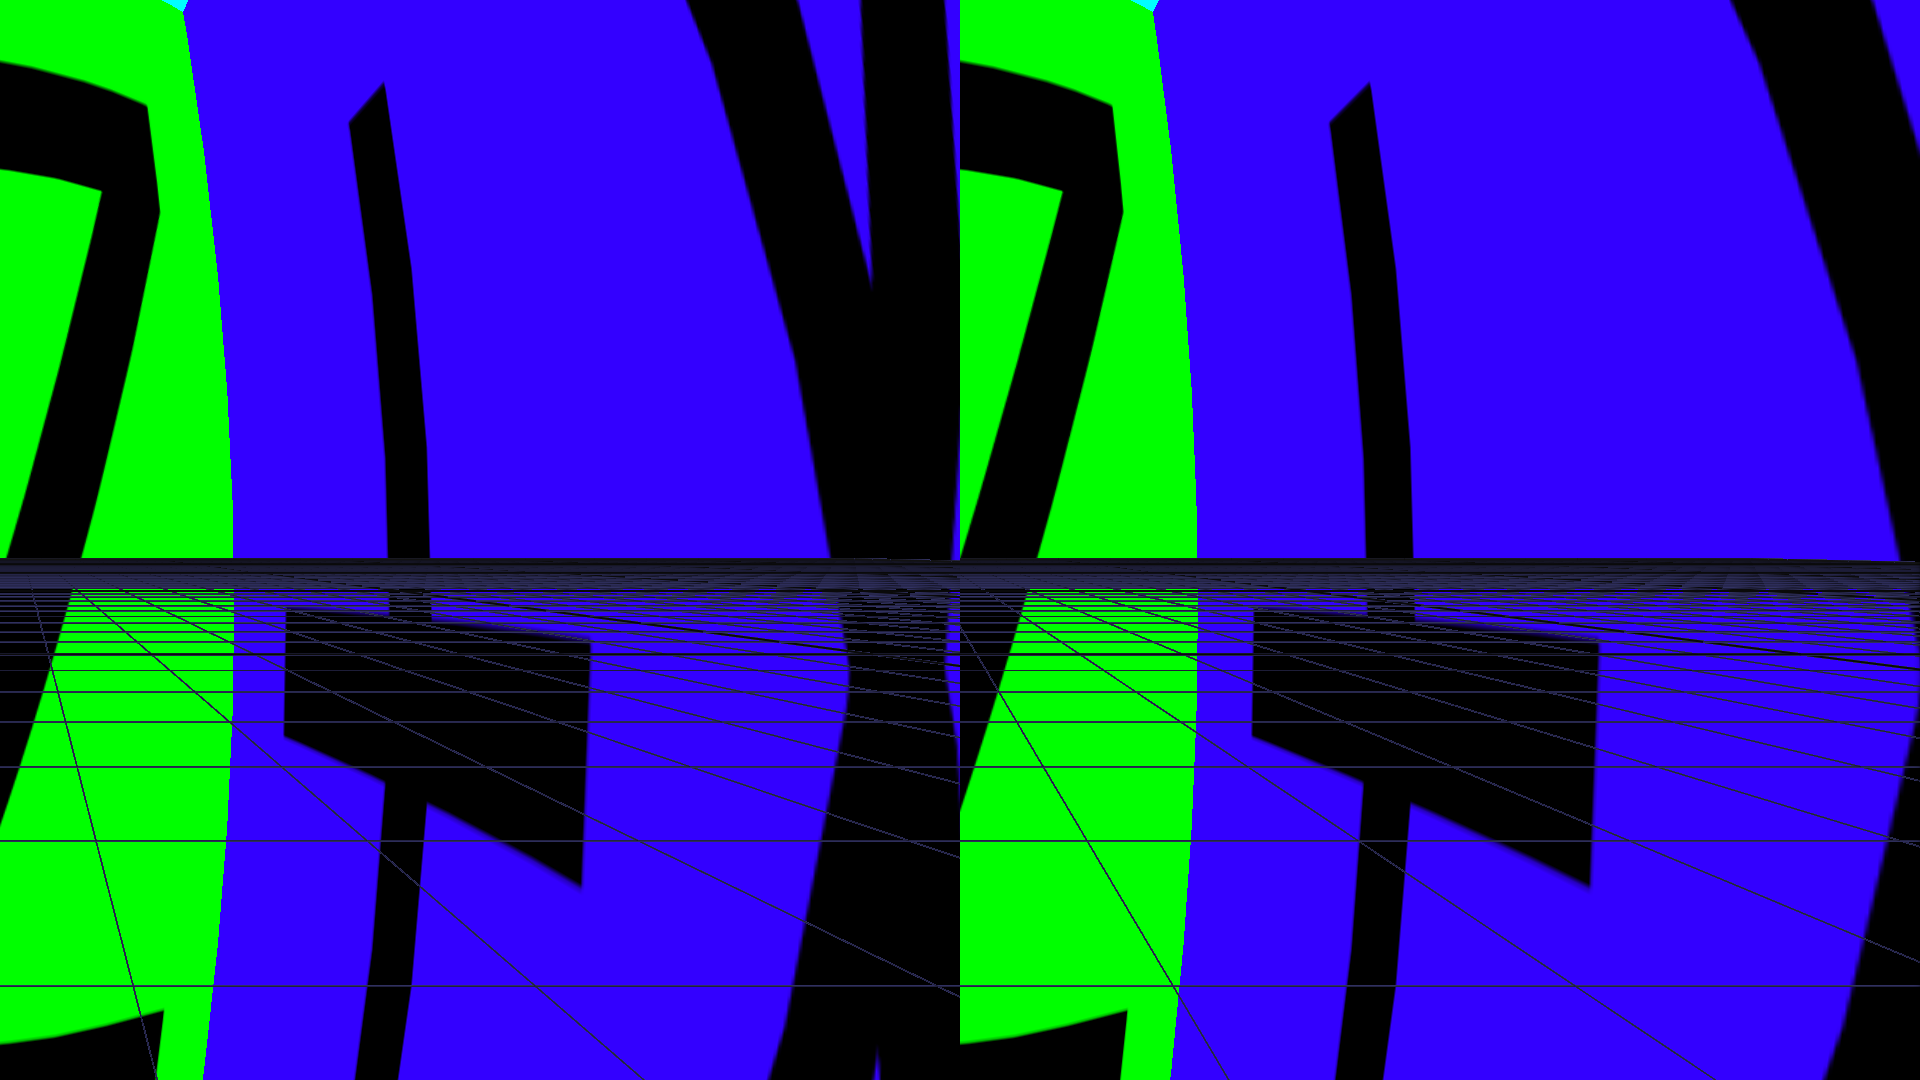
\includegraphics[width=0.45\linewidth,keepaspectratio=true]{figs/right_screen.png}\\
(a) Left display & 
(b) Right display
\end{tabular}
\caption{Vertical split of the stereo views.}
\label{fig.split_screens}
\end{figure}

The complete pipeline is described by Figure~\ref{fig.osg_pipeline}, where each box is a transformation. The bigger boxes are the view and projection transforms, $M_{cam}$ and  $M_{hcp}$, common for both screens. The smaller boxes are the transformations that specific for each screen and have different parameters, $M_{eye}$ and $M_{tilt}^{T}$ after $M_{cam}$; $M_{stereo}$ and $M_{off}$ after $M_{hcp}$.

\begin{figure}[!htb]
\centering
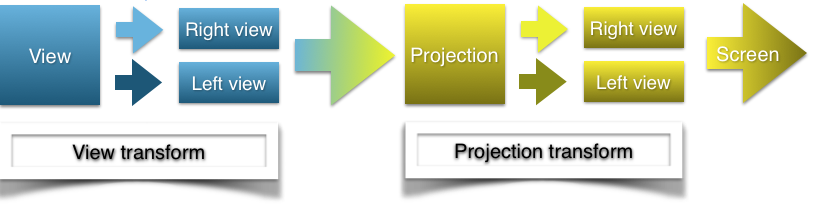
\includegraphics[width=0.9\linewidth,keepaspectratio=true]{figs/osg_pipeline.png}
\caption{The viewing pipeline for right and left views.}
\label{fig.osg_pipeline}
\end{figure}

%\section{Holographic Projection}
\label{sec.hologram_projection}

In the proposed holographic projection, the perspective projection is computed in a similar way, a 3D point in a truncated pyramid frustum (eye coordinates) is mapped to NDC; and the range of $x$ and $y$-coordinates from respectively $[l, r]$ and $[b, t]$ are still mapped to $[-1, 1]$, but the $z$-coordinate is mapped in the inverse way, from $[n, f]$ to $[1, -1]$. 

Note that the eye coordinates are still defined in the right-handed coordinate system, but now the camera at the origin is looking along $+Z$ axis in eye space, and along $+Z$ axis in NDC. The inversion of the $Z$  axis in Figure~\ref{fig.new_projection01} can be achieve by negating the third column of the projection matrix in Equation~\ref{eq.projection_matrix}.

%Since glFrustum() accepts only positive values of near and far distances, we need to negate them during the construction of \verb|GL_PROJECTION| matrix.

\begin{figure}[h!]
\centering
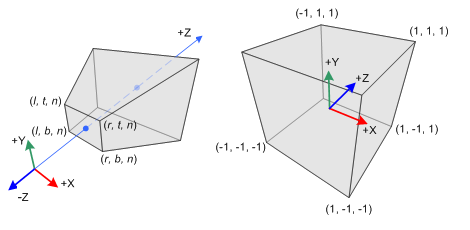
\includegraphics[width=0.9\linewidth,keepaspectratio=true]{figs/new_gl_projectionmatrix01.png}
\caption{Perspective Frustum and Normalized Device Coordinates (NDC)}
\label{fig.new_projection01}
\end{figure}


%The following diagrams show how a point $(x_e, y_e, z_e)$ in eye space is projected to $(x_p, y_p, z_p)$ on the near plane.

%\begin{figure}[!ht]
%\centering
%\begin{tabular}{cc}
%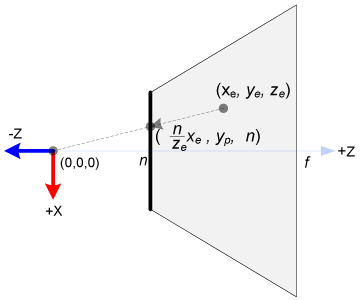
\includegraphics[width=0.45\linewidth,keepaspectratio=true]{figs/new_gl_projectionmatrix03.png}&
%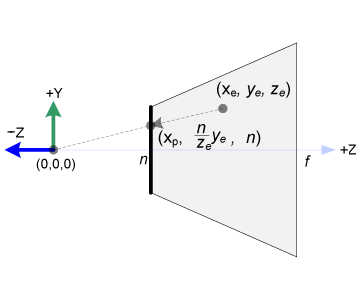
\includegraphics[width=0.45\linewidth,keepaspectratio=true]{figs/new_gl_projectionmatrix04.png}\\
%Top View of Frustum&
%Side View of Frustum
%\end{tabular}
%\caption{Views of the frustum.}
%\label{fig.new_frustum}
%\end{figure}

The permuted projection matrix is; 
\begin{equation}
\begin{aligned}
M^{\prime}_{proj} &= 
\begin{pmatrix} 
\frac{2n}{r-l} & 0 & -\frac{r+l}{r-l} & 0 \\
0 & \frac{2n}{t-b} & -\frac{t+b}{t-b} & 0 \\
0 & 0 & \frac{(f+n)}{f-n} & \frac{2fn}{f-n} \\
0 & 0 & 1 & 0 \\
\end{pmatrix} \\
\end{aligned}
\end{equation}

